% Flight Plan: one-page run sheet for the paper plane KPI game in Class 23 (instructor only; it reveals the lesson).
% Kept out of git by the root .gitignore until after section B. Button names (\btn) match host.html and
% snap.html as deployed Nov 10, 2026.
\documentclass[10pt,letterpaper]{article}

\usepackage[margin=0.35in]{geometry}
\usepackage[T1]{fontenc}
\usepackage{palatino,mathpazo}
\usepackage{amssymb}
\usepackage{xcolor}
\usepackage{multicol}
\usepackage{enumitem}
\usepackage{tabularx}
\usepackage{tikz}
\usepackage[colorlinks=true, urlcolor=cyan, linkcolor=cyan]{hyperref}
\usepackage{url}
\urlstyle{same}

\definecolor{miami}{RGB}{195,20,45}
\definecolor{soft}{RGB}{248,236,238}
\definecolor{tip}{RGB}{245,158,11}
\pagestyle{empty}
\setlength{\parindent}{0pt}
\setlength{\columnsep}{0.22in}
\setlist{nosep, leftmargin=*, topsep=0pt}
\setlength{\tabcolsep}{3pt}
\setlength{\multicolsep}{2pt}

\newcommand{\hd}[1]{\par\smallskip{\color{miami}\small\bfseries #1}\par\vspace{1pt}}
\newcommand{\key}[1]{{\setlength{\fboxsep}{0.8pt}\fbox{\ttfamily\bfseries #1}}}
\newcommand{\btn}[1]{{\setlength{\fboxsep}{0.8pt}\fbox{\sffamily #1}}}
\newcommand{\site}{isa401-flight-plan.vercel.app}
\newcolumntype{L}{>{\raggedright\arraybackslash}X}

\begin{document}
\small

\begin{center}
	{\Large\bfseries Flight Plan: Run Sheet}\\[1pt]
	{\small ISA 401, Class 23, Wed Nov 11, 2026 (A 8:30, B 10:05). During design, never say whether a KPI matters and never comment on a design.}
\end{center}

\vspace{-4pt}
\begin{tabularx}{\textwidth}{@{}lL@{}}
	\hline
	\textbf{Students} & \url{https://\site/?section=A} \quad and \quad \texttt{?section=B} \quad (QR codes on the game slide) \\
	\textbf{Projector} & \url{https://\site/host?section=A}: runs everything; \key{Space} = next step \\
	\textbf{Phone} & \url{https://\site/snap?section=A}: only takes the board photo \qquad \textbf{Key:} the Game Day word \qquad \textbf{Test:} \texttt{?section=Z} \\
	\hline
\end{tabularx}

\hd{1. Before class}
\begin{minipage}[t]{0.63\textwidth}
\begin{itemize}[label=$\square$]
	\item Draw the X at chest height; mark the 6 ft throw line.
	\item \textbf{X width:} tape it from the left end of the strokes to the right end (diagram). Draw it \textbf{12 in wide} and you type nothing; otherwise enter it in \btn{Settings} $\rightarrow$ X width (in).
	\item Markers: black, blue, red, green, purple. Tape measure. A sheet of paper in your pocket.
	\item Projector: open, enter the key, \btn{Reset} twice. \btn{Music}: pick the four Rocky files on \texttt{M:}.
	\item Phone: open the snap page, enter the key.
	\item \textbf{Before B:} erase the marks (keep the X); switch projector and phone to B; \btn{Reset} twice.
\end{itemize}
\end{minipage}\hfill
\begin{minipage}[t]{0.35\textwidth}
\vspace{0pt}
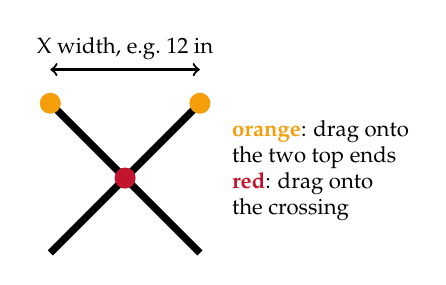
\begin{tikzpicture}[scale=0.95]
	\draw[line width=2.6pt] (-1,-1) -- (1,1); \draw[line width=2.6pt] (-1,1) -- (1,-1);
	\fill[miami] (0,0) circle (4pt);
	\fill[tip] (-1,1) circle (4pt); \fill[tip] (1,1) circle (4pt);
	\draw[<->, thick] (-1,1.45) -- (1,1.45) node[midway, above, font=\footnotesize] {X width, e.g.\ 12 in};
	\node[font=\footnotesize, anchor=west, align=left] at (1.3,0.1) {\textcolor{tip}{\textbf{orange}}: drag onto\\the two top ends\\\textcolor{miami}{\textbf{red}}: drag onto\\the crossing};
\end{tikzpicture}\\[-2pt]
{\footnotesize On the check screen, the handles sit on the same two ends you taped. That distance sets inches per pixel.}
\end{minipage}

\hd{2. Phase by phase}
{\renewcommand{\arraystretch}{1.05}
\begin{tabularx}{\textwidth}{@{}l@{\hspace{4pt}}c@{\hspace{6pt}}L@{\hspace{6pt}}L@{}}
	\hline
	\textbf{Phase} & \textbf{min} & \textbf{What you click} & \textbf{Say / watch} \\
	\hline
	Slides + Lobby & 4 & Deck: KPI slide, game slide. Projector: \btn{Lobby} & Teams = seating rows. \\
	Design & 17 & \btn{Design}: clock + music start; \btn{+ 1 min} / \btn{$-$ 1 min} & Tiles show counts only. Stay silent on relevance. \\
	Vote & 7 & Read each team's accuracy definition; \btn{Lock the rule} (tie: Override menus) & One vote per student. A miss is never 0 (0 = dead center). \\
	Throws & 12 & \btn{Next team}; tap a throw for \btn{missed board}; \btn{Change} sets a team's marker & 3 throws per team from 6 ft. No two teams can share a marker. \\
	Check & 2 & Phone: \btn{First photo}, \btn{Take photo}. Projector: \btn{Pre-fill with AI}, fix marks, \btn{Save marks} & Each team ``3 of 3''. AI down: click the marks yourself. \\
	Reveal & 4 & \btn{Reveal}; \btn{Show the measurement} & Winner's brief; ``would the winner change?'' \\
	Instructor & 4 & No team made a ball: \btn{Instructor}, \btn{Start my throws}, 3 throws, phone \btn{Second photo}, marks, \btn{Score my throws}. Teams did: tick each one, \btn{These teams did it} & Win: mic-drop GIF + Final Bell. Lose: music cuts, airball GIF. \\
	KPIs & 8 & \btn{KPIs} & Each team's KPIs by bucket, next to the ball. \\
	After-game deck & 6 & Open \texttt{23b\_after\_the\_game.html}, then back to the main deck & Baggage claim, ethics cases, jobs. \\
	\hline
\end{tabularx}}
\smallskip
About 64 min, so the report slides get about 16. Behind? \btn{$-$ 1 min} on Design, or shorten KPIs.

\hd{3. The metrics table}
\colorbox{soft}{\parbox{\dimexpr\textwidth-2\fboxsep}{%
\begin{tabularx}{\linewidth}{@{}Lll@{\hspace{10pt}}|@{\hspace{6pt}}Lll@{}}
	\textbf{Product (client)} & \textbf{Relevance} & \textbf{Ball} & \textbf{Operational} & \textbf{Relevance} & \textbf{Ball} \\
	\hline
	Accuracy: distance to the X & tied to the goal & best & Cycle time (build one plane) & process & $\sim$5 s \\
	Consistency / spread & tied to the goal & tight & Takt time (available time / planes needed) & process & met \\
	Hit rate within N in & tied to the goal & & Lead time (design start to ready) & process & $\sim$5 s \\
	Reaches the board & tied to the goal & every throw & People involved & process & 1 \\
	Durability & supports the goal & unlimited & Cost of resources (incl.\ scrapped) & process & 1 sheet \\
	Skill needed to throw & supports the goal & none & Prototypes / iterations & process & 0 \\
	Unit cost (final plane) & client might value & 1 sheet & Training time & process & none \\
	Aesthetics & client might value & \textbf{loses} & \multicolumn{3}{l@{}}{\textit{No match: you discuss.} Cost is in both lists.} \\
	Speed, flight time, distance & not tied & \textbf{loses} & & & \\
	Weight & not tied & & & & \\
\end{tabularx}}}

\raggedcolumns
\begin{multicols}{2}
\hd{4. If students complain}
Tape the throw and type the inches in its \btn{Tape (in)} box on the Reveal screen. The board shows both numbers and re-ranks with a note. The \btn{Ruler} (click two points on the photo) checks the photo in front of them.

\columnbreak
\hd{5. After class}
\begin{itemize}[label=$\square$]
	\item After section B ends: \btn{Publish recap} in A and in B.
	\item \btn{Settings} $\rightarrow$ \btn{Export CSV} for the 0.15 bonus (the winning team gets it either way).
	\item Remove the Class 23 lines from \texttt{.gitignore}; push the decks. Reset Z.
\end{itemize}
\end{multicols}

\end{document}
